%    Programmable logic devices
% notes:
%~~~~~~~~~
%------------------------------------------------------------------------------------------------------
% Setting path to image 
\graphicspath{{../src/PLO/img/}}

\lstset{ %
  language=VHDL,                         % choose the language of the code
  basicstyle=\small,              % the size of the fonts that are used for the code: basicstyle=\small, \footnotesize
  backgroundcolor=\color{White},         % choose the background color. You must add \usepackage{color}
  commentstyle=\color{help}\textit,
  stringstyle=\ttfamily,                 % typewriter type for strings
  keywordstyle=\color{keyword}\textbf,
  breaklines=true,                       % sets automatic line breaking
  breakatwhitespace=true,                % sets if automatic breaks should only happen at whitespace
  showspaces=false,                      % show spaces adding particular underscores
  showstringspaces=true,                 % underline spaces within strings
  showtabs=true,                         % show tabs within strings adding particular underscores
  frame=none,	                           % adds a frame around the code - none, single
  tabsize=8,                             % sets default tabsize to 8 spaces
  captionpos=b,                          % sets the caption-position to bottom
  numbers=left,                          % where to put the line-numbers -none, left, right
  numberstyle=\footnotesize,             % the size of the fonts that are used for the line-numbers
  stepnumber=1,                          % the step between two line-numbers. If it's 1 each line
                                         % will be numbered
  xleftmargin=3em,                       % adjust left margin
}
%------------------------------------------------------------------------------------------------------
% file CPP.tex
%=====================================Kapitola: Přehled jazyka C++=====================================
  %================Kapitola: Architektura programovatelných logických obvodů=========================
\chapter{Architektura}
\minitoc
\newpage
  \section{Typy struktur programovatelných logic\-kých obvodů}
    Programovatelný logický obvod nebo programovatelné logické zařízení, často také \texttt{PLD}
    (\emph{programmable logic device}) nebo \texttt{FPD} (\emph{Field-Programmable Device}), je
    elektronická součástka (obvod) používaná pro vytváření digitálních obvodů. Na rozdíl od hradel,
    registrů a jiných digitálních obvodů není funkce zařízení tohoto druhu v době výroby ještě
    definovaná. Než může být PLD použito, musí být nejprve naprogramováno.
    
    \subsection{Historie}
      Historické kořeny moderních programovatelných polí jsou v prvních progra\-mo\-va\-tel\-ných
      pamětech typu \texttt{PROM} (\emph{firma Radiation, 1970}) a jejich zákaznicky
      programovatelných verzím \texttt{EPROM} (\emph{Intel, 1971}) a \texttt{EEPROM} (\emph{Intel,
      1978}). Paměť \texttt{PROM} lze využít pro realizaci kombinačních logických funkcí tak, že
      paměť využijeme jako tzv. \emph{vyhledávací tabulku} \textbf{LUT} (angl. \emph{Lookup
      Table}). V tomto případě přivádíme na adresové vodiče \texttt{PROM} paměti vstupní signály
      (proměnné). Obsah paměti \texttt{PROM} vytvoříme tak, že na adresy jejichž hodnota je tvořena
      vektorem hodnot vstupních proměnních uložíme hodnoty, které jsou tvořeny vektory požadovaných
      výstupních hodnot. Výstupní datové signály paměti \texttt{PROM} pak reprezentují výstupy
      kombinančí logiky. Tímto způsobem můžeme např. paměti \texttt{PROM} o velikosti 2 Kb s
      organizací 256x8 bitů (8 adresových vodičů, 8 datových vodičů), vytvořit programovatelný
      logický obvod, kterým lze realizovat 8 kombinačních funkcí s 8 vstupními signály
      (proměnnými). Výhodou takovéto realizace je, že všechny realizované funkce mají stejné
      zpoždění ze vstupu na výstup a to pro všechny možné kombinace vstupních hodnot. Na principu
      generátorů logických funkcí pomocí pamětí (\texttt{LUT}) je založena funkce obvodů
      \texttt{FPGA}.
      
      Permanentní paměti, jako takové, ale neumožňovaly úspornou realizaci logické fun\-kce. Mezi
      první programovatelné logické obvody lze zařadit obvody \texttt{PLA} (angl.
      \emph{Programmable Logic Array}), neboť v roce 1970 společnost \texttt{Texas Intruments - TI}
      podařilo vyvinout maskou programovatelný integrovaný obvod \texttt{TMS2000}, založený na
      paměti \texttt{ROAM} (angl. \emph{Read Only Associative Memory}) společnosti \texttt{IBM}.
      \texttt{TMS2000} disponoval 17 vstupy, 18 výstupy s 8 \texttt{JK} klopnými obvody. Obvod bylo
      možné programovat modifikací vodivé propojovací masky během výroby (tj. koncový uživatel jej
      nemohl programovat). Obvody \texttt{PLA} obsahovaly pole hradel \texttt{AND} následované
      polem hradel \texttt{OR}. Logická funkce tedy vznikala v disjunktivní formě, tj. jako součet
      součinů. Tento způsob tvorby logickék funkce se uchytil a na tomto principu je založena
      funkce dnešních obvodů architektur \texttt{SPLD} a \texttt{CPLD}. Nicméně se tyto obvody na
      trhu příliš neprosadily.
      
      Vývoj však pokračoval dál a v roce 1975 přišla na trh firma \texttt{Signetics Corporation} s
      obvody nazvanými \texttt{FPLA} - (\emph{Field Programmable Logic Array}), konkrétně se
      jednalo o obvod 82S100. Po převzetí firmy Signetics firmou \texttt{Philips} byl tento obvod
      označován také jako PLS100. Obvody \texttt{FPLA} tvořilo programovatelné pole \texttt{AND}
      následnované programovatelným polem hradel \texttt{OR}. Tyto obvody však měly poměrně dlouhou
      dobu přenosu signálu ze vstupu na výstup. Pro návrh obvodů neexistoval žádný jazyk, a tak
      musel návrhář nastavovat přímo hodnoty jednotlivých programovatelných buňek. Tyto nevýhody
      spolu s poměrně vysokou cenou způsobili malé rozšíření těchto obvodů.
      
      Dalším významným krokem bylo uvedení obvodů \texttt{PAL} - (\emph{Programmable Logic Array}).
      Tyto obvody navrhla firma \texttt{MMI - Monolithic Memories, Inc} v roce 1978. Obvody
      \texttt{PAL} vycházeli z obvodů \texttt{FPLA} a obsahovaly programovatelné pole hradel
      \texttt{AND}, které bylo následováno pevným neprogramovatelným polem hradel \texttt{OR}. Ke
      každému hradlu \texttt{OR} tak bylo možno připojit pouze omezený počet výstupů hradel
      \texttt{AND} (součinů). Díky tomuto zjednodušení došlo ke snížení doby přenosu signálu ze
      vstupu na výstup. Oba tyto typy obvodů \texttt{FPLA} i \texttt{PLA} byly totiž založeny na
      bipolární PROM technologii s programovatelnými pojistkami tzv. \emph{fusible-link}.
      Programování bylo realizováno vstříknutím dostatečně velkého náboje, který způsobil přepálení
      vybrané vnitřní pojistky. Zbývající neporušené pojistky se staly součástí implementovaného
      číslicový obvodu. Pojistky ovšem zvyšují zpoždění signálu v obvodu, zvětšují složitost a ve
      výsledku i cenu. Počet součinů, které byly připojeny na vstup hradla \texttt{OR}, byl na
      základě praktických zkušeností stanoven na osm. Velkou výhodou těchto obvodů bylo, že se daly
      programovat v tehdy již běžných programátorech pamětí \texttt{PROM}. Mezi první obvody řady
      \texttt{PAL} patří například \texttt{PAL16L8} (kombinační výstupy) a \texttt{PAL16R8}
      (výstupy s registry).
      
      Firma \texttt{MMI} dále napsala pro tyto obvody návrhový software, který umožňoval popsat
      číslicový systém pomocí velmi jednoduchého jazyka ve formě booleovských rovnic a z něj pak
      vygenerovat výstup, jímž bylo možné obvody \texttt{PAL} naprogramovat. Tím došlo k významnému
      zjednodušení vlastního návrhu obsahu těchto obvodů. Tento software se jmenoval
      \texttt{PALASM} (\emph{PAL Assembler}) a firma \texttt{MMI} ho zveřejnila ve formě zdrojového
      kódu napsaného v jazyce \texttt{FORTRAN}. Program \texttt{PALASM} umožňoval dokon\-ce
      softwarovou simulaci navrženého obvodu. Díky funkcím návrhu a simulace  lze \texttt{PALASM}
      označit za první návrhový systém pro \texttt{PLD} obvody. Všechny zmíněné obvody dnes řadíme
      do první generace \texttt{PLD}obvodů. Za zmínku ještě stojí, že firmy \texttt{Signetics
      Corporation} a \texttt{MMI} již mezi dnešními výrobci programovatelných obvodů nenajdeme.
      
      Vývoj v oblasti \texttt{PLD} obvodů pokračoval a postupně se začaly objevovat nové
      \texttt{PLD} obvody, které řadíme již do druhé generace. V roce 1983 uvedla firma
      \texttt{AMD} (\emph{Advanced Micro Devices}) obvod \texttt{PAL22V10}. Tento obvod byl založen
      na obvodech \texttt{PAL} popsaných v předchozím odstavci, přinesl však jedno významné
      vylepšení, a to tzv. \textbf{výstupní makrobuňku} (\texttt{OLMC} - angl. \emph{Output Logic
      Macro Cell}). Tyto obvody bývají označovány jako obvody \texttt{PAL} s makrobuňkou. Výstupní
      makrobuňka byla umístěna na každém výstupu obvodu. Každou makrobuňku bylo možné naprogramovat
      buď jako kombinační nebo registrový výstup. Dále blo možné u jakékoliv makrobuňky
      programovat, zda má být výstup v přímé nebo negované formě. Výstup makrobuňky byl třístavový,
      ovládaný jedním logickým součinem, což umož\-ňo\-va\-lo přepnutí makrobuňky z výstupního
      režimu do funkce vstupu. Tento typ obvodu vyrábělo svého času kromě firmy \texttt{AMD} mnoho
      dalších firem, např. \texttt{Cypress Semiconductor}, \texttt{Lattice Semiconductor} a
      \texttt{Texas Instruments}.
      
      Všechny dosud zmíněné obvody měly jednu nevýhodu - byly programovatelné pou\-ze jednou
      (\texttt{OTP} - \emph{One Time Programmable}). Díky rozvoje technologie u pamětí
      \texttt{EPROM} se dostala tato technologie i do oblasti \texttt{PLD} obvodů a tudíž se na
      trhu objevili \texttt{PLD} obvody, jejichž obsah bylo možné smazat pomocí ultrafialového
      záření - obvody lze opakovaně mazat a znovu programovat.
      
      V roce 1984 vstoupila na scénu firma \texttt{DATA I/O} se svým návrhovým systémem
      \textbf{ABEL}, jenž disponoval jazykem vyšší úrovně, určený pro popis číslicových systémů
      (\texttt{HDL} - \emph{Hardware Description Language}), který byl nazván stejně jako návrhový
      systém, tj \texttt{ABEL} - \emph{Advanced Boolean Expression Language}. Jazykem \texttt{ABEL}
      lze popsat číslicový systém pomocí booleovských rovnic, pravdivostní tabulky a stavových
      automatů, přičemž tyto způsoby je možné kombinovat. Práva na jazyk \texttt{ABEL} získala po
      několika akvizicíh firma \texttt{XILINX}. Tento jazyk již sedmou revizi a dodnes ho některé
      současné návrhové systémy podporují (např. Xilinx a Lattice Semiconductor). Pro návrh nových
      číslicových systémů založených na \texttt{PLD} obvodech se však doporučuje používat některý z
      novějších \texttt{HDL} jazyků, např. jazyk \texttt{VHDL} nebo jazyk \texttt{Verilog}.
      
      Další vývoj \texttt{PLD} obvodů pokračoval s nástupem technologie pamětí \texttt{EEPROM} a
      jejím využítí v \texttt{PLD} obvodech. Této nové technologie bylo využito zejména u
      \texttt{PLD} obvodů označovaných jako \texttt{GAL} - \emph{Generic Array Logic}. Obvody
      \texttt{GAL} lze zařadit do třetí generace \texttt{PLD} obvodů. Obvody typu \texttt{GAL} jsou
      také zařazovány do třídy jednoduchých programovatelných obvodů (\texttt{SPLD}).
      
      Na konci osmdesátých let minulého století nastává v oblasti \texttt{PLD} obvodů bouřlivý
      vývoj. Vývojem a výrobou \texttt{PLD} se na konci osmdesátých a začátkem devadesátých let již
      zabývá mnoho firem a vývoj \texttt{PLD} obvodů již nelze od této doby přehledně rozdělit ani
      stručně popsat. V průběhu tohoto období vznikají nové řady \texttt{PLD} obvodů, nazývané
      \texttt{CPLD} - \emph{Complex Programmable Logic Device}. Jmenujme např. alespoň obvody
      \texttt{MACH} firmy \texttt{AMD} a dále vznik první řady obvodů \texttt{MAX}, kterou společně
      vyvinula firma \texttt{ALTERA} a \texttt{Cypress Semiconductor}. Nové obvody v této době na
      trh uvádí také firma \texttt{XILINX} (řady \texttt{XC7200} a \texttt{XC7300}),
      \texttt{QuickLogic}, \texttt{Lattice Semiconductor} a tak by bylo možné pokračovat dál a dál.
      Z uvedeného je vidět, že cesta vývoje \texttt{PLD} obvodů nebyla a není ani dnes nijak
      přímočará a byla navíc od svých počátků provázena soudními spory firem o patentová práva a
      tato situace trvá dodnes.
      
      Lze však řicí, že od začátku devadesátých let vyvíjí většina firem dvě od sebe velmi odlišné
      architektury \texttt{PLD} obvodů. První je architektura \texttt{CPLD} obvodů, založená na
      programovatelné matici hradel \texttt{AND}, hradlech \texttt{OR} a makrobuňkách (vychází tedy
      z původní koncepce obvodů \texttt{PAL})  a na programovatelných místech používá buňky
      \texttt{EEPROM} nebo \texttt{FLASH}.
      
      Kvůli rostoucí velikosti obvodů se začalo později místo rozšiřování logických funkcí užívat
      spíše skládání více matic PLD obvodů do jednoho pouzdra. Vznikly tak obvody, které dnes
      nazýváme \texttt{CPLD} (\emph{Complex Programmable Logic Device, Altera, 1988}). Od
      \texttt{CPLD} byl už pak jen malý krok k prvním \texttt{FPGA} obvodům (\emph{Xilinx, 1984}).
      Dnes dostupná \texttt{FPGA} se ovšem od architektur z poloviny osmdesátých let významně
      odlišují. Trendem je pozvolný příklon k hrubozrnným architekturám; obvodům, které kromě
      elementárních programovatelných logických bloků obsahují také další komplexní podpůrné bloky.
      
    \newpage
    \subsection{Obvody typu Simple Programmable Logic Device}  
      \subsubsection{Programmable Read Only Memory (PROM)}\label{PLO_kap_PROM}
        Po mnoho let nebyly obvody \texttt{PROM} \emph{Programmable Read Only Memory} zařazovány do
        skupiny programovatelných logických obvodů, ačkoliv většina nejmenších PROM (např. 32x8)
        byly používány jako logické prvky (dekodéry, převodní tabulky kódů, znakové generátory).

        \begin{figure}[ht!]
          \centering
          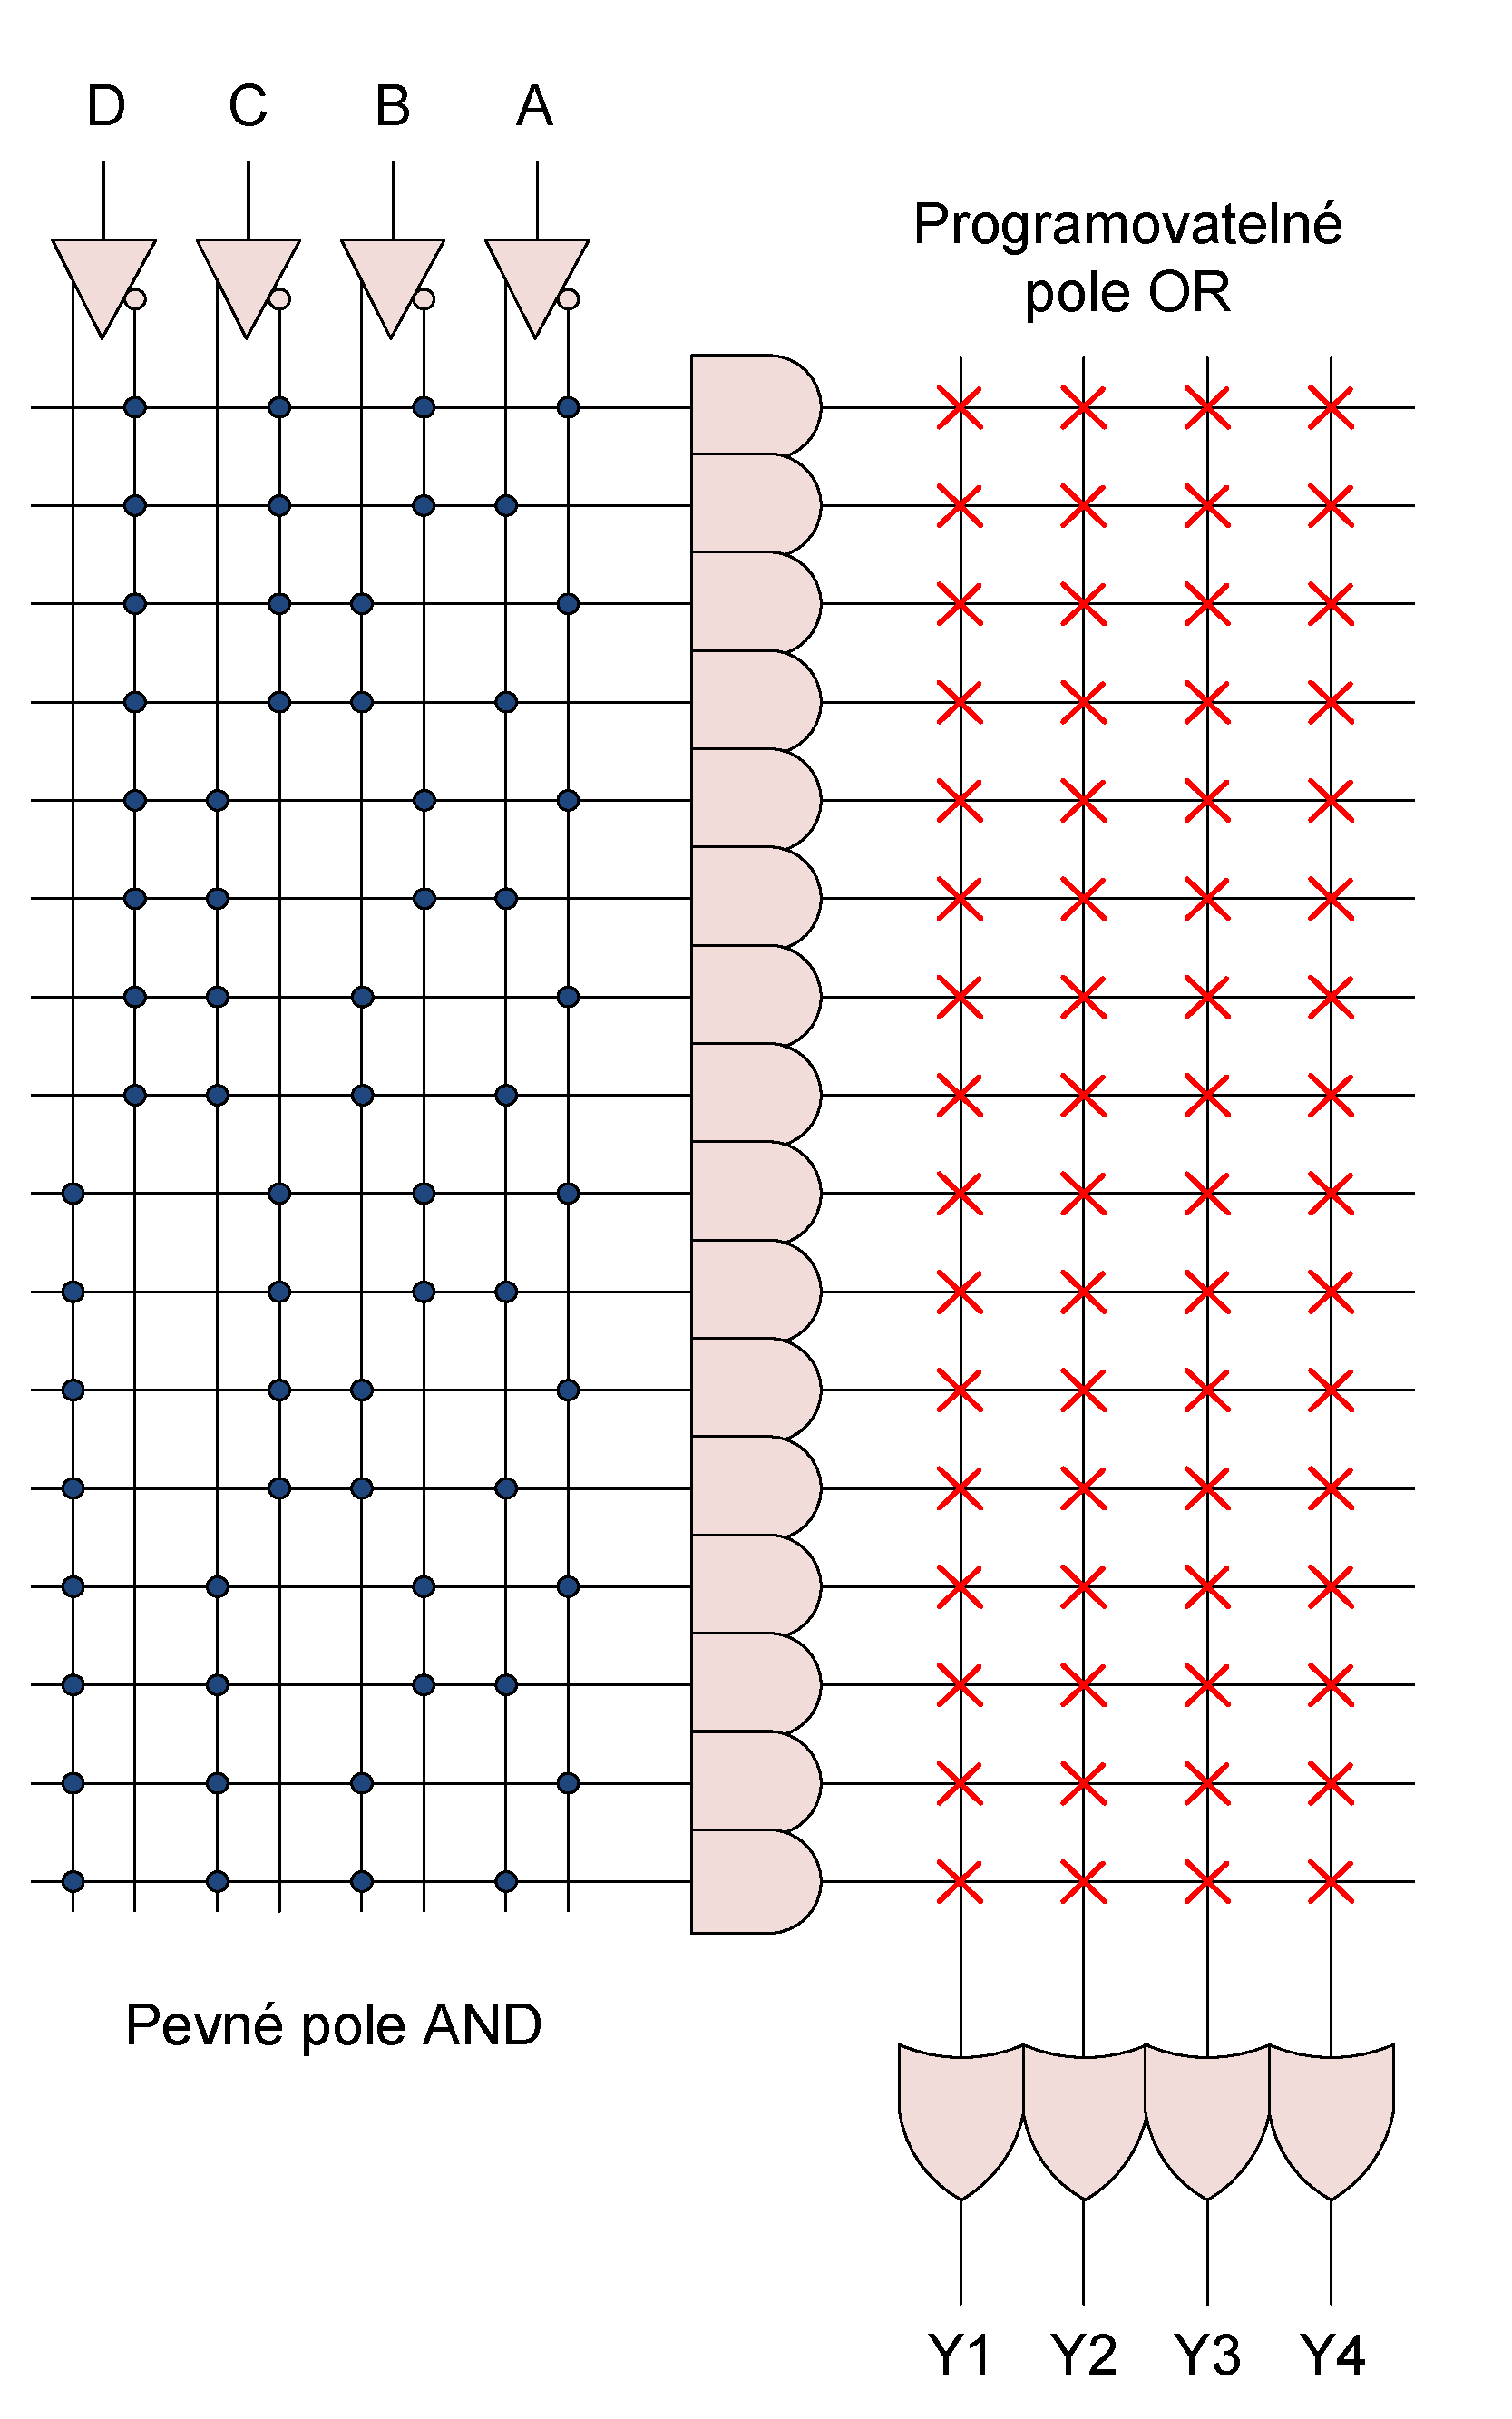
\includegraphics[width=\linewidth]{architektura_PROM.pdf}
          \caption[Architektura PROM]{PLD typu Programmable Read Only Memory (PROM)}
          \label{PLO:fig_arch_PROM}
        \end{figure}
        
        Obvody \texttt{PROM} představuje matici paměťových buněk, jejíž řádky jsou adresovatelné
        vstupní signály a datové sloupce představují výstupní signály. Počet adresových a datových
        signálů determinuje rozměr matice. Např. 4 vstupní signály umožňují adresaci 16 řádků, 4
        datové signály indikují, že každý řádek se skládá ze 4 pamě\-ťo\-vých buněk. Z pohledu
        architektury obvodů PLD obsahují PROM pevné propojovací pole hradel \texttt{AND},
        následované programovatelným polem hradel \texttt{OR} (viz obr. \ref{PLO:fig_arch_PROM})

        \begin{figure}[ht!]
          \centering
          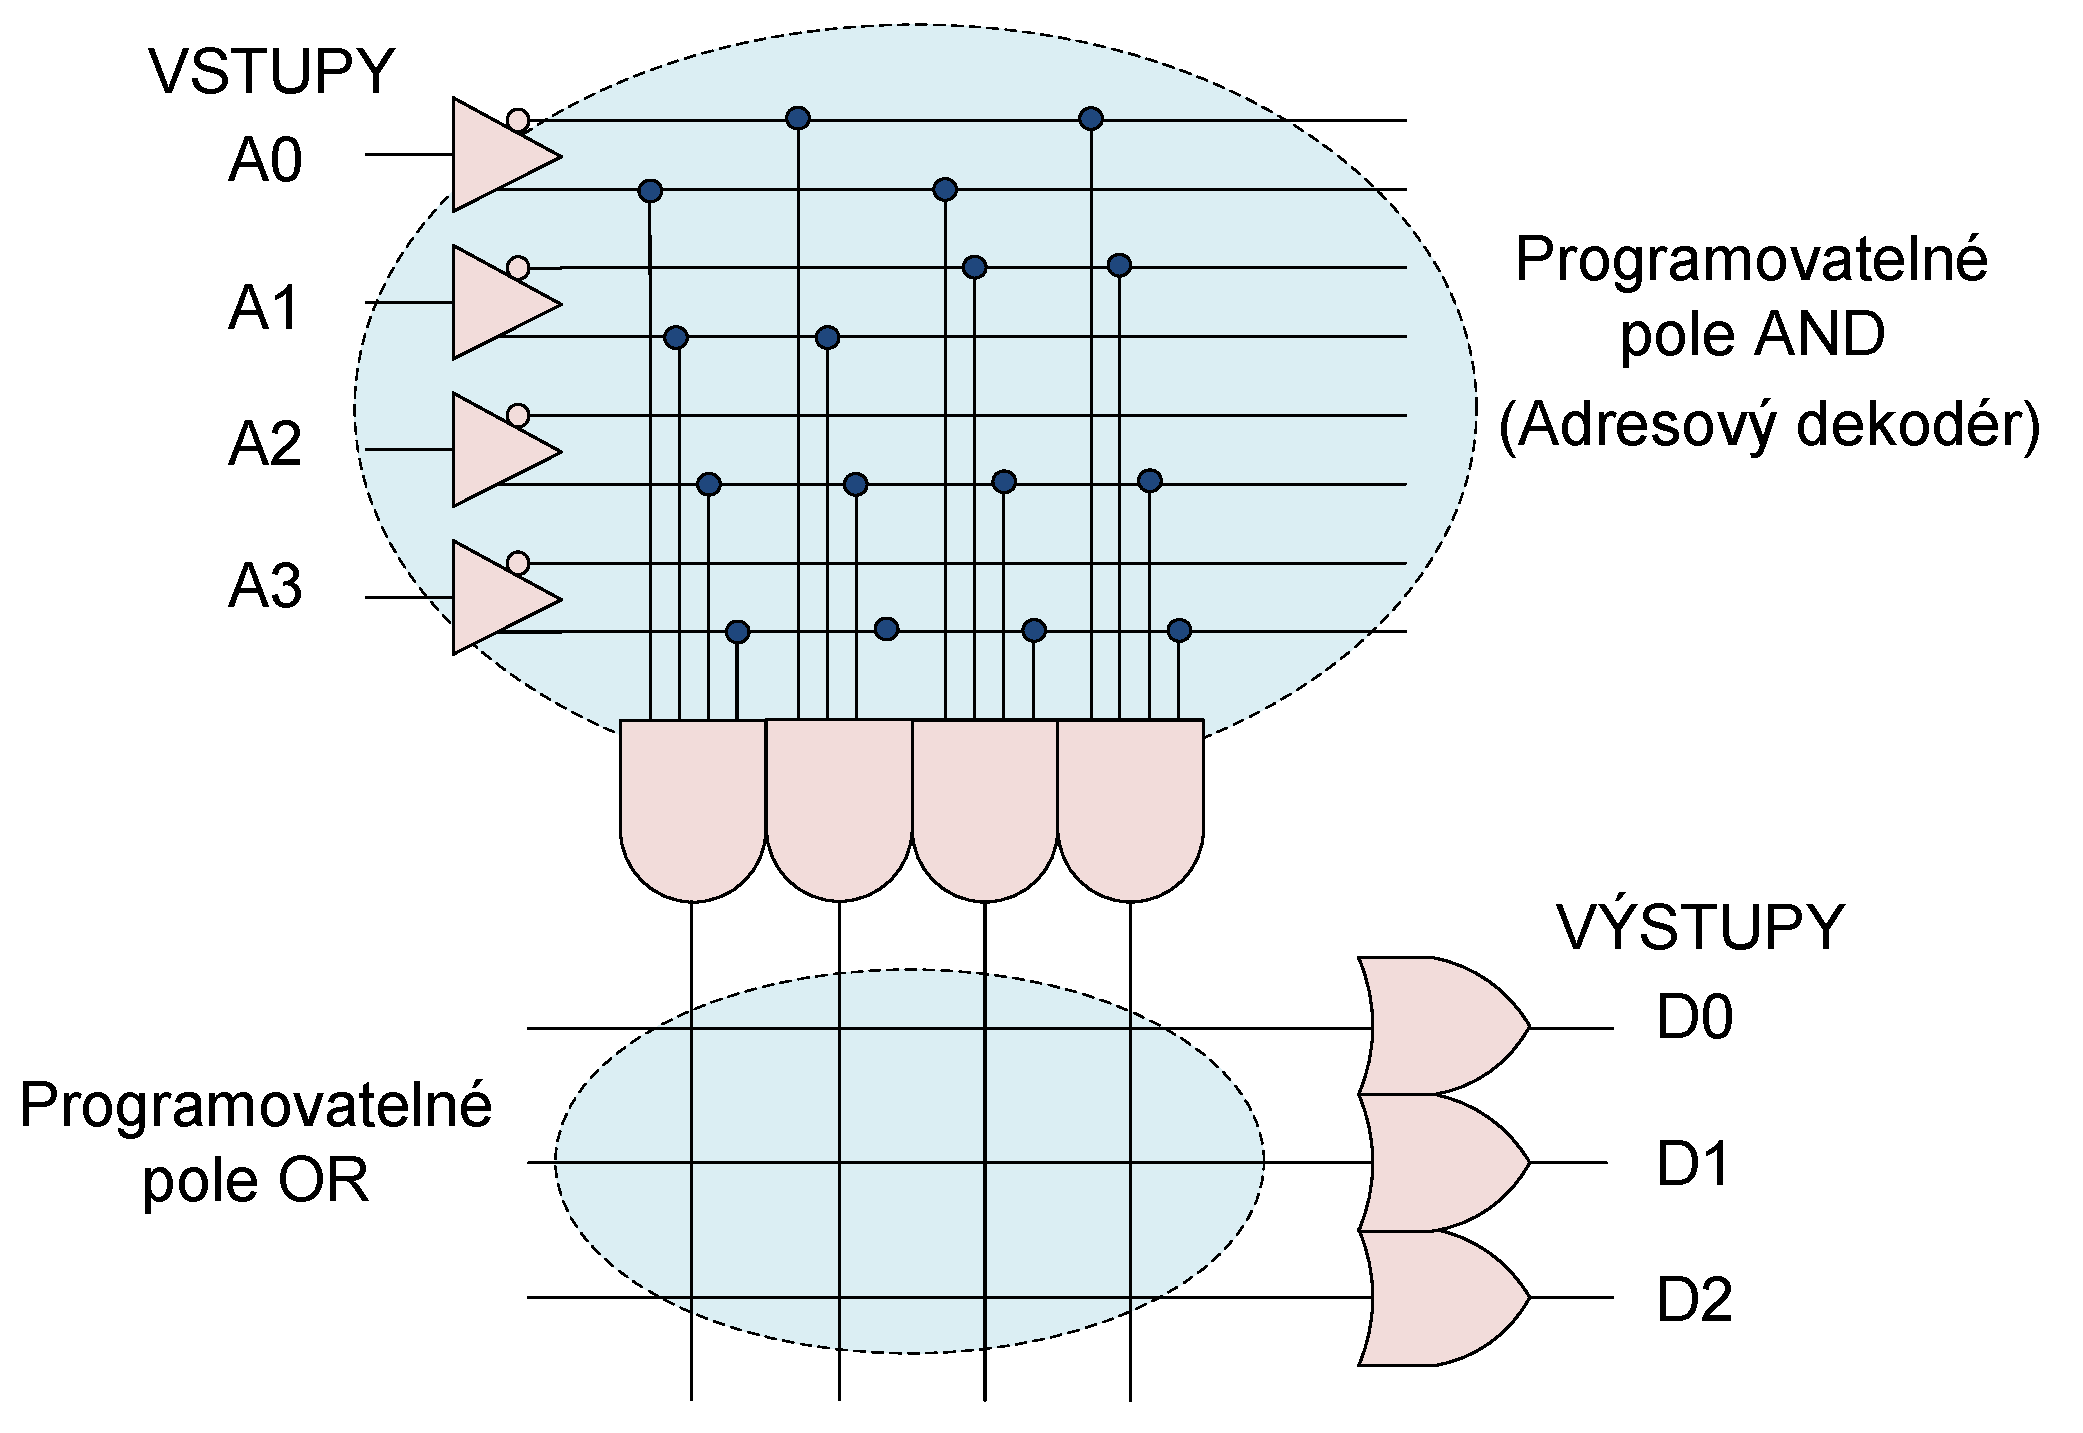
\includegraphics[width=0.9\linewidth]{schema_PROM.pdf}
          \caption[Schéma obvodu PROM]{Schéma obvodu PROM}
          \label{PLO:fig_sch_PROM}
        \end{figure}      

        Všeobecně platí, že obvody PROM jsou nejvhodnějším kandidátem implementace takových
        aplikací, které vyžadují, aby na každou kombinaci vstupních signálů byla jiná odezva
        výstupních signálů. Překážkou je omezení počtu vstupních signálů, eventuálně je limitující
        také velikost programovatelné matice. Její velikost se přidá\-ním nového vstupu vždy
        zdvojnásobí (omezení počtu vstupních signálů jistým způsobem řeší obvody typu PAL viz kap.
        \ref{PLO_kap_PAL})\cite[s.~59]{PLD_Grada}.
      
        Na obr. \ref{PLO:fig_sch_PROM} je uvedena architektura obvodu PROM prostřednictvím
        symboliky obvodů PLD. Každý term odpovídá jedné z jeho adres. Programovatelná hradlo OR
        odpovídají datovým bitům obvodu PROM (výstupní slovo). Např. PROM velikosti 32x8
        představuje obvod PLD s 5 vstupy, 32 součinovými termy ($32=2^5$) a 8 programovatelnými
        výstupními OR hradly.

     \subsubsection{PLD typu Programmable Logic Array (PLA)}\label{PLO_kap_FPLA}
        Obvody \texttt{PLA}(\emph{Programmable Logic Array}) patří k průkopníkům v oblasti
        programovatelných logických polí. Obsahují programovatelné pole hradel AND a zároveň i
        programovatelné pole hradel OR (viz obr. \ref{PLO:fig_arch_FPLA}).
        Vstupní signály jsou přivedeny v přímém i invertovaném stavu do pole AND hradel.
        \begin{figure}[ht!]
          \centering
          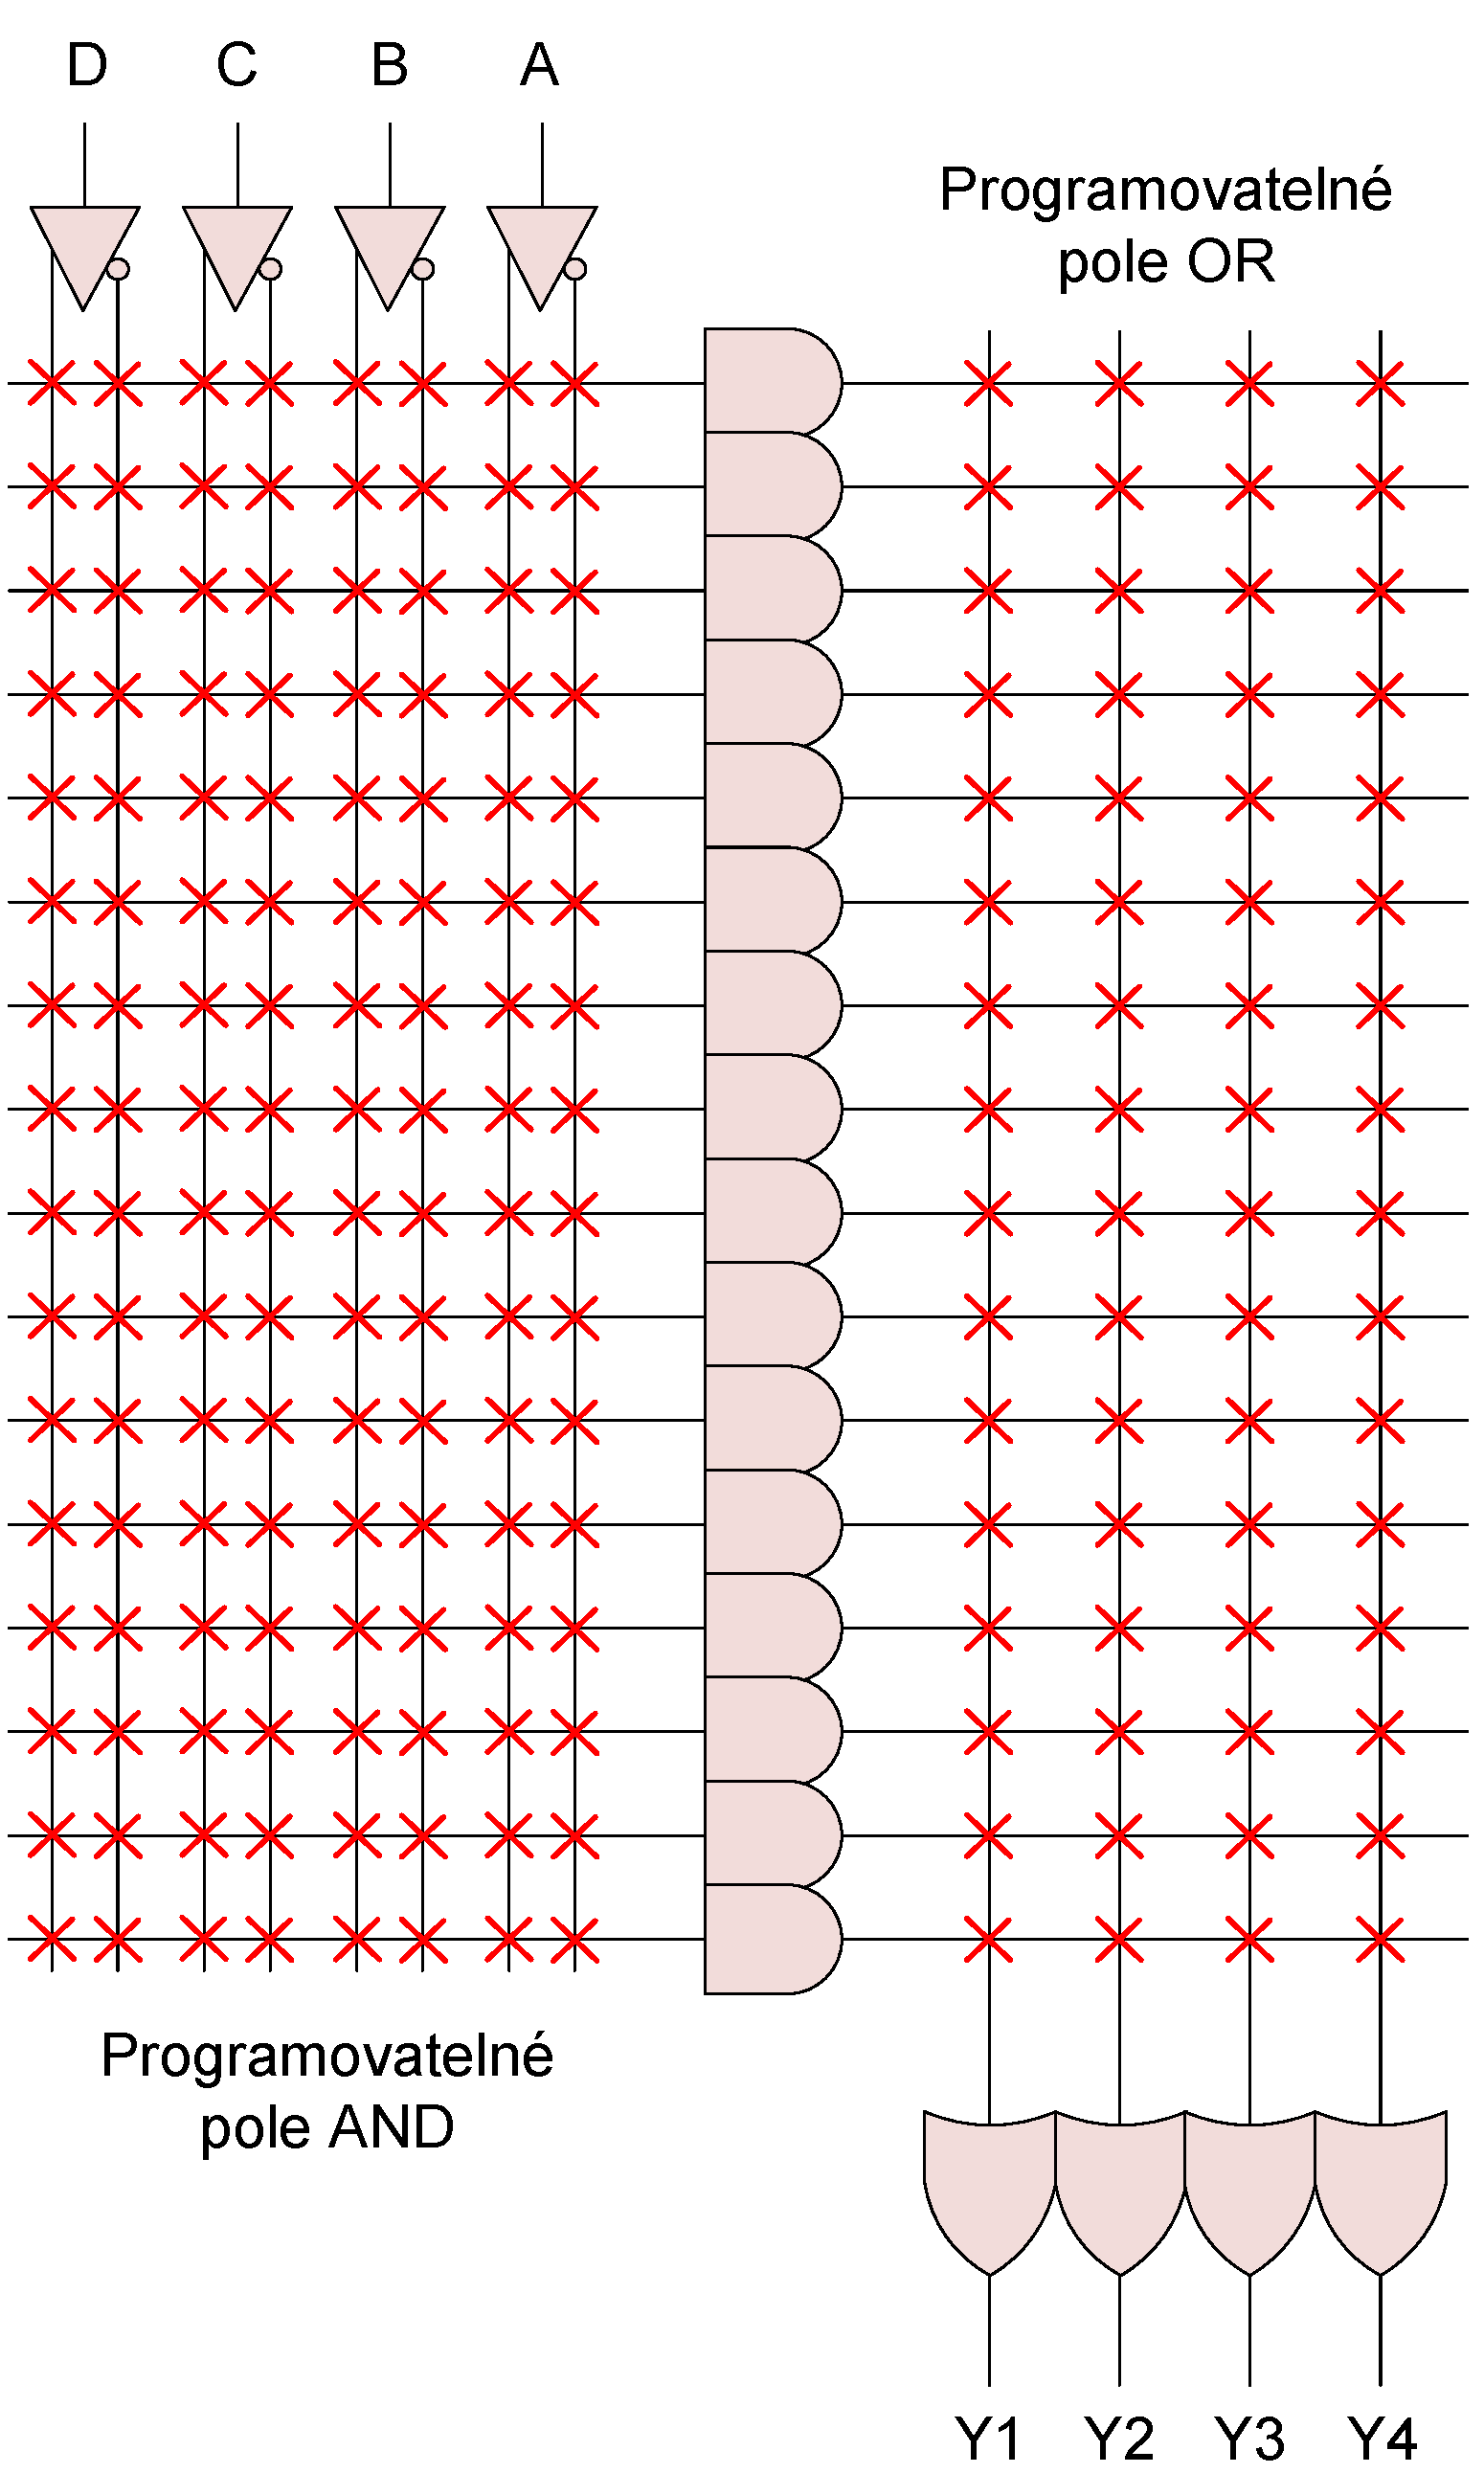
\includegraphics[width=\linewidth]{architektura_FPLA.pdf}
          \caption[Architektura obvodů PLA]{Architektura obvodů PLA}
          \label{PLO:fig_arch_FPLA}
        \end{figure}
        
        Oproti obvodům \texttt{PROM}, mají obvody \texttt{PLA} toto pole programovatelné, takže je
        možné snadno vytvořit součinové termy z libovolné kombinace vstupních (přímých i
        negovaných) signálů. Součinové termy jsou přivedeny do programovatelného pole OR hradel,
        které umožňuje připojení libovolného termu k libovolnému hradlu OR. Jeden term může být
        přiveden na vstup i několika hradel OR. Na jejich výstupu je formována požadovaná logická
        funkce ve tvaru "součtu součinů".

        Je-li obvod PLD vybaven programovatelným polem AND, jako je tomu u obvodů \texttt{PLA} (a i
        např. u PAL kapitola \ref{PLO_kap_PAL}), může být využita pouze polovina programovatelných
        spínačů propojovacího pole. Tato skutečnost je zřejmá, protože vstupní signály jsou do pole
        přivedeny v přímém i invertovaném tvaru a v žádném součin se nemůže současně vyskytovat
        přímý i invertovaný signál (součin by vždy nabýval hodnoty logická nula). Takže nejméně
        polovina (a v praxi i více, protože všechny součiny vždy neobsahují všechny veličiny) není
        při konstrukcích logických funkcí využita. Je tedy zřejmé, jak neefektivně je využita
        plocha křemíkového čipu, na kterém je obvod typu PLA realizován. Tato skutečnost stimuluje
        další vývoj a vznik nových architektur obvodů PLD \cite[s.~63]{PLD_Grada}.
        
     \subsubsection{PLD typu Programmable Array Logic (PAL)}\label{PLO_kap_PAL}
        Obvody typu PAL jsou dalším z typů programovatelných logických obvodů. Jsou to PLD obvody s
        programovatelným polem hradel AND a pevným poler hradel OR. K jednomu hradlu OR lze
        připojit pouze omezený počet součinových termů, přičemž nelze současně jeden term připojit
        k několika hradlům OR.
      
        \begin{figure}[ht!]
          \centering
          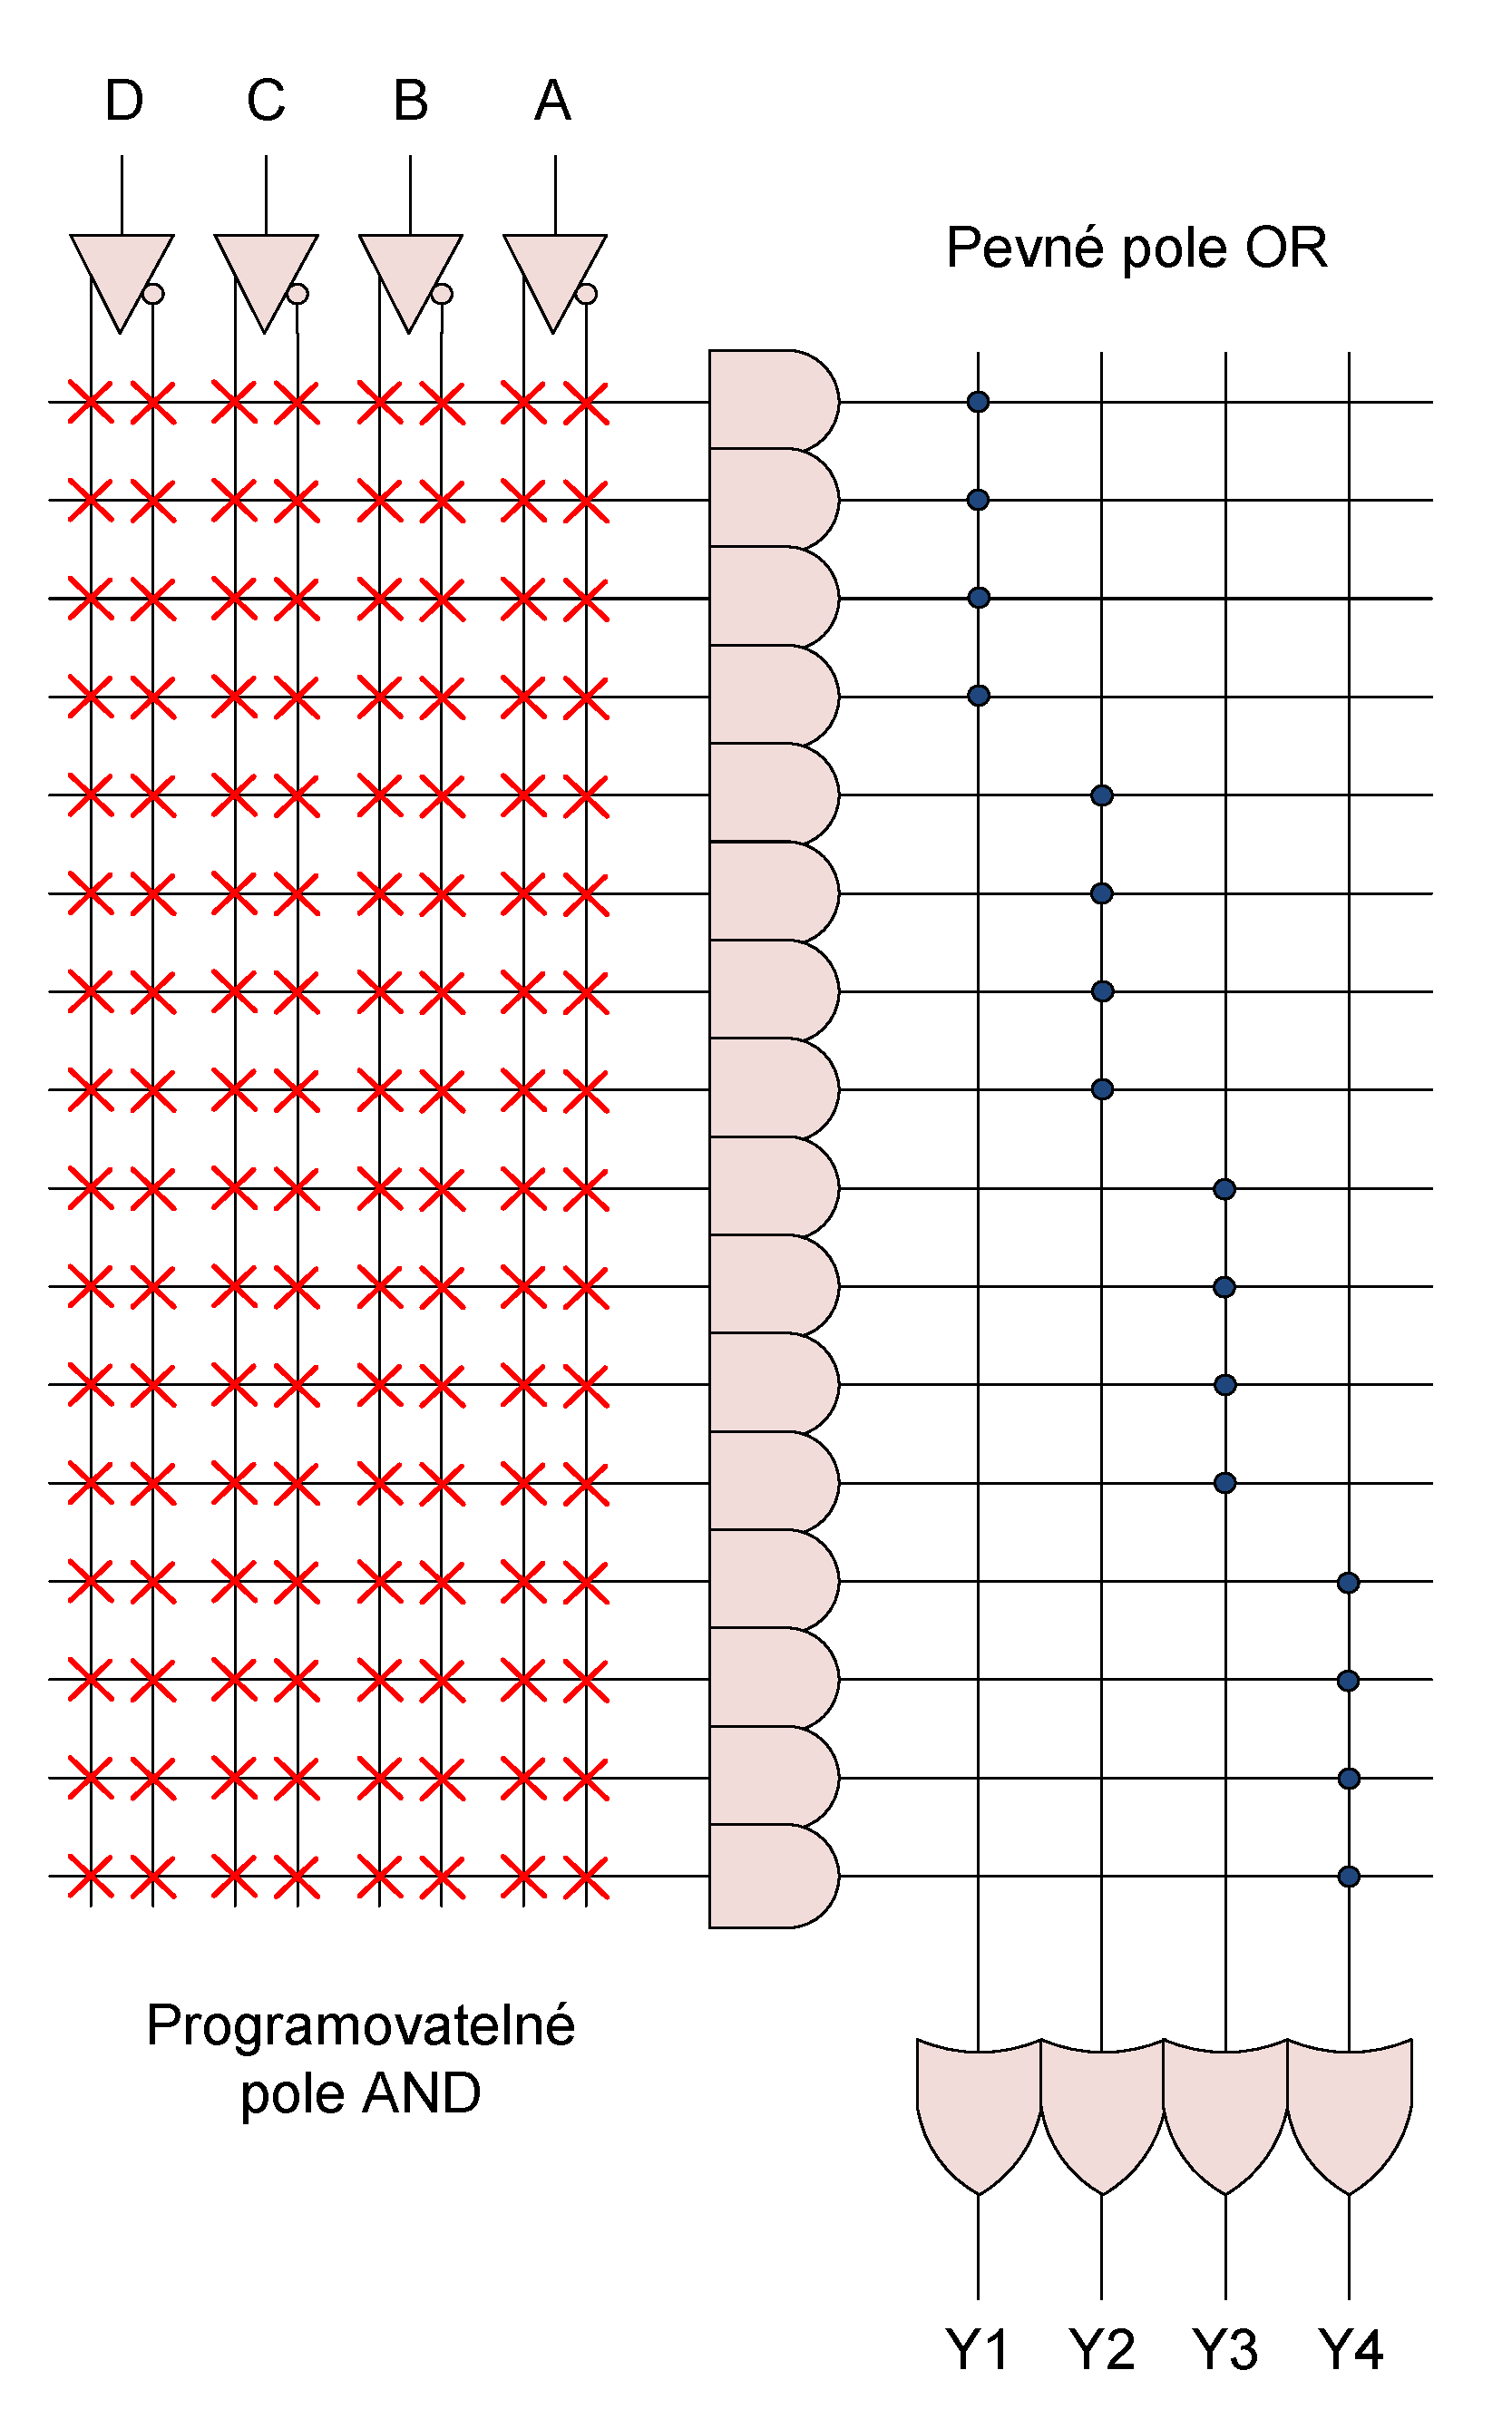
\includegraphics[width=\linewidth]{architektura_PAL.pdf}
          \caption[Architektura obvodů PAL]{Architektura obvodů PAL}
          \label{PLO:fig_arch_PAL}
        \end{figure}
        
        Jednodušší architektura oproti v té době existujícím FPLA obvodům, umožnila zkrácení doby
        přenosu signálu. Obvody PAL byly navrženy tak, aby "vypadaly" jako standardní obvody PROM a
        mohly tak být programovány standardními programátory obvodů PROM. Tím se výrobci obvodů PAL
        vyvarovali požadavků na dodatečné vývojové prostředí, jak tomu bylo v době uvedení na trh v
        případě FPLA obvodů.
        
     \subsubsection{PLD typu Simple Programmable Logic Device - \texttt{SPLD}}\label{PLO_kap_GAL}
       Obvody typu \texttt{GAL} (\emph{Generic Array Logic}) patří do skupiny elektricky
       reprogramovatelých obvodů PLD (\texttt{EEPLD} - \emph{Electrically Erasable Programmable
       Logic Device}). Z hlediska klasifikace PLD obvodů lze obvody \texttt{GAL} charakterizovat
       jako obvody s programovatelným polem AND hradel a pevným polem hradel OR. Významná
       od\-liš\-nost od obvodů PAL spočívá v možnosti elektrického reprogramování a využití
       makro\-buň\-ky (Output Logic Macrocell) na výstupech obvodu.
       
        \begin{figure}[hb!]
          \centering
          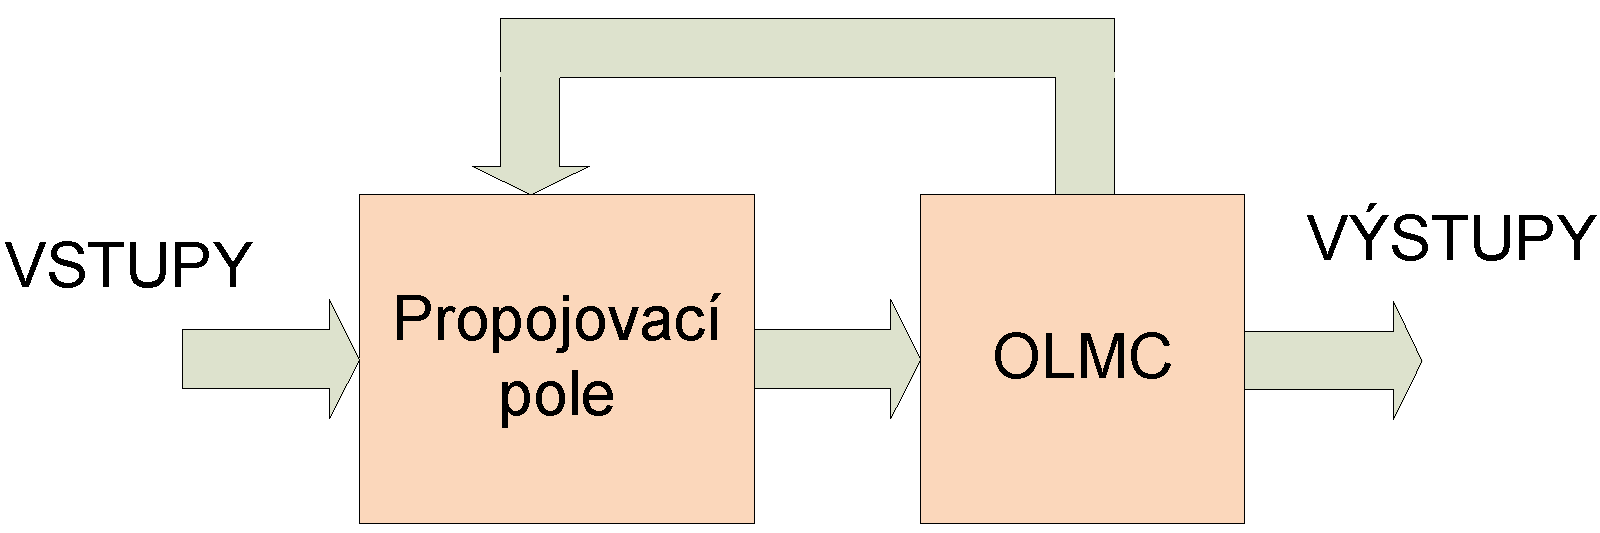
\includegraphics[width=0.7\linewidth]{architektura_GAL.pdf}
          \caption[Struktura obvodu GAL]{Obecná struktura obvodu \texttt{GAL}}
          \label{PLO:fig_arch_GAL}
        \end{figure}
               
  \newpage
  \subsection{Obvody typu Complex Programmable Logic Device - \texttt{CPLD}} 
    Obvody typu \texttt{CPLD} patří podobně jako obvody \texttt{SPLD} do skupiny elektricky
    reprogramovatelných \texttt{PLD} obvodů (\texttt{EEPLD}). Většina \texttt{CPLD} obvodů je
    programovatelná v cílovém systému, nesou tedy i označení \texttt{ISP} (\emph{In-system
    programming}). Tyto obvody jsou typické, podobně jako obvody \texttt{GAL}, svou
    programovatelnou maticí hradel AND následovanou hradlem OR a makrobuňkou. Na výstupu hradla OR
    je tak stejně jako u obvodů \texttt{GAL} formována pořadovaná logická funkce ve tvaru
    \emph{součtu součinů}. Od obvodů GAL se však obvody CPLD liší hlavně velkým centrálním
    propojovacím polem. Makrobuňky jsou sdruženy do větších skupin a tvoří tzv. \textbf{funkční
    bloky} \cite[p~279]{Pinker2006}. Pro architekturu obvodů CPLD jsou charakteristické tyto čtyři
    struktury:
    \begin{itemize}
      \item velké centrální propojovací pole (\emph{Global Routing Pool}),
      \item programovatelné funkční bloky  (\emph{Generic Logic Block - GLB}), uspořádané ko\-lem
            propojovacího pole, sestávající z:
        \begin{itemize}
          \item programovatelné matice AND,
          \item několika makrobuňek,
          \item alokátoru součinů,          
        \end{itemize}
      \item výstupní propojovací pole (\emph{Output Routing Pool - ORP}),
      \item vsutpní/výstupní bloky  (\emph{I/O Blocks}).  
    \end{itemize}

        \begin{figure}[hb!]
          \centering
          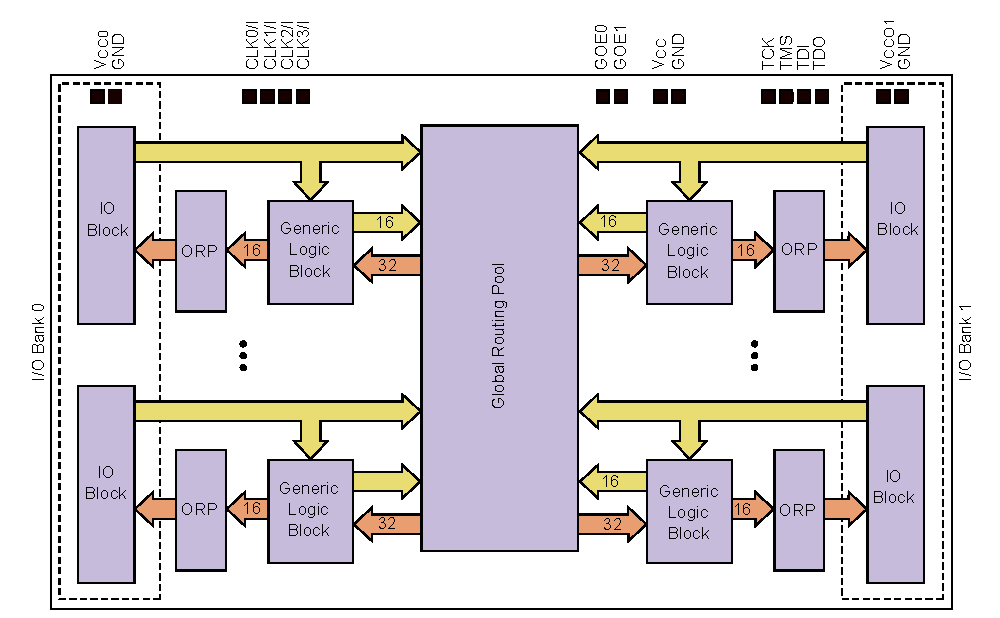
\includegraphics[width=1\textwidth]{PLD_ispMACH4000_arch.pdf}
          \caption[Struktura obvodu CPLD]{Architektura \texttt{CPLD ispMACH4000} společnosti
                                          \texttt{Lattice}}
          \label{PLO:fig_arch_ispMACH4000}
        \end{figure}  
            
    Všechny výše uvedené stavební prkvy mají u různých výrobců různá označení, jejich význam a
    funkce je však velmi podobná. Pomocí makrobuňek lze realizovat různě složité kombinační a
    sekvenční logické či paměťové funkce. Přes programovatelné \textbf{vstupní/výstupní bloky} lze
    přivádět vstupní signály z vývodů obvodu nebo naopak vyvádě výstupní signály. Na rozdíl od
    jednodušších SPLD, kde vstupní/výstupní obvody jsou přímo spojeny s makrobuňkou, jsou však u
    CPLD zásadně od makrobuňek odděleny a tvoří samostatný I/O blok, do kterého mohou výstupní
    signály z makrobuňek vstupovat přes programovatelné \textbf{výstupní propojovací pole}. Tím se
    všeobecně zlepší využítí jak makrobuňek, tak výstupních obvodů.
    
    Všechny vstupní/výstupní bloky a všechny makrobuňky lze spolu vzájemně propojit pomocí
    \textbf{centrálního programovatelného propojovacího pole}.

        \begin{figure}[ht!]
          \centering
          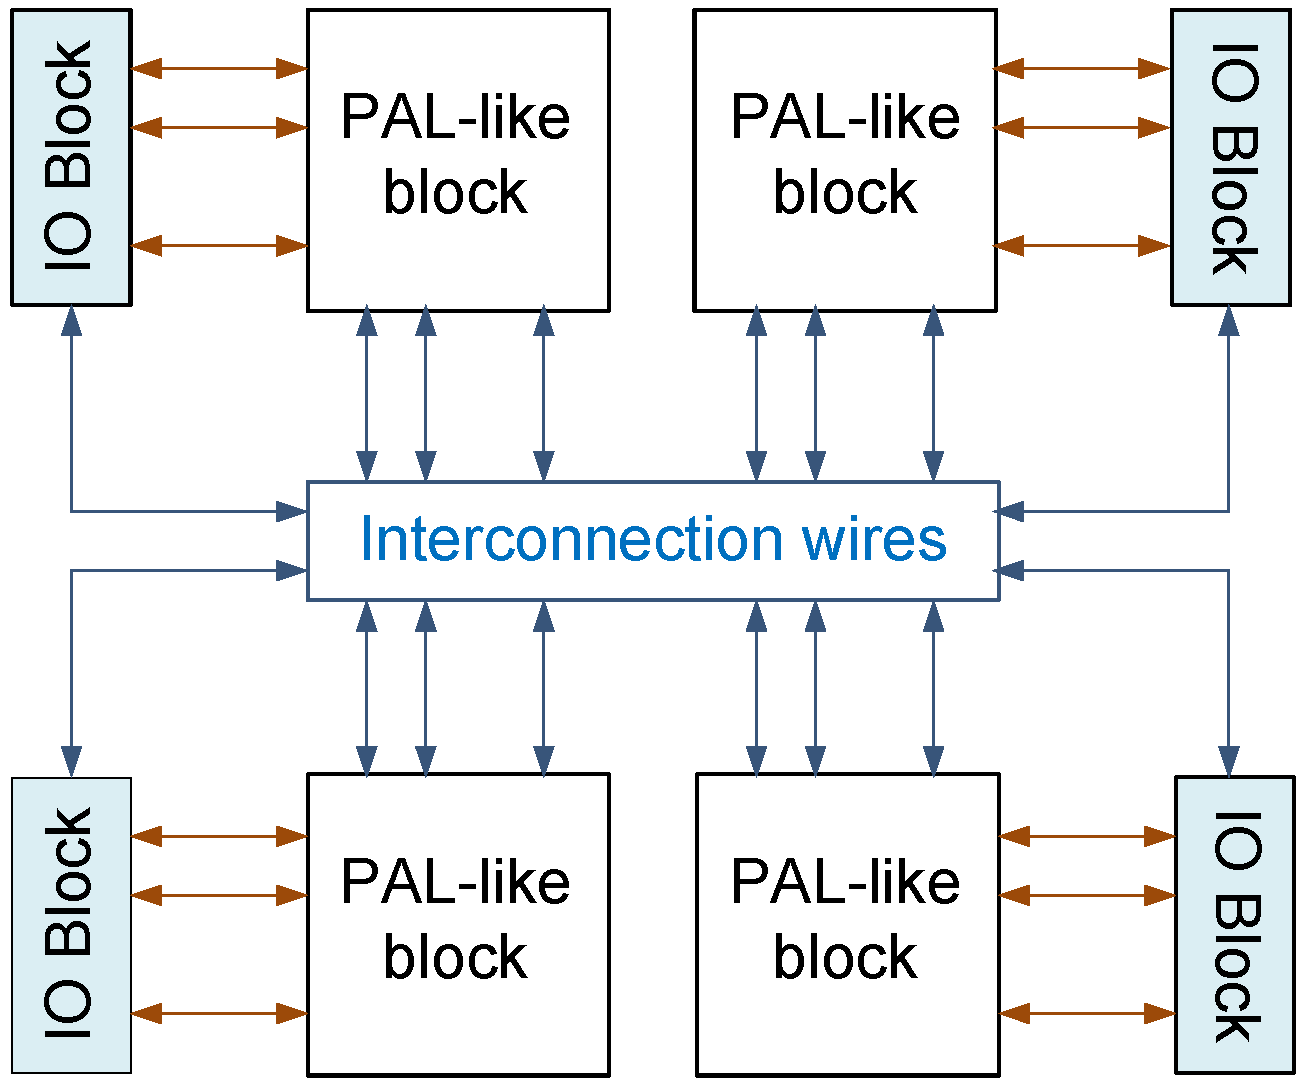
\includegraphics[width=0.9\linewidth]{architektura_CPLD.pdf}
          \caption[Struktura obvodu CPLD]{Obecná struktura obvodu CPLD}
          \label{PLO:fig_arch_CPLD}
        \end{figure} 
           
  \newpage
  \subsection{Obvody typu Field-Programmable Gate Array - \texttt{FPGA}}   
    \newpage
    \subsection{Terminologie}
      \begin{itemize}
        \item \textbf{PLA} — \emph{Programmable Logic Array} nebo také \textbf{FPLA} \emph{Field
              Programmable Logic Array}: Obvod obsahuje matici \texttt{AND} za nímž následuje matice
              \texttt{OR}, jež jsou obě programovatelné.
              % is a relatively small FPD that contains two levels of logic, an AND-plane and an
              % OR-plane, where both levels are programmable (note: although PLA structures are
              % sometimes embedded into full-custom chips, we refer here only to those PLAs that are
              % provided as separate integrated circuits and are user-programmable).
        \item \textbf{PAL} - \emph{Programmable Array Logic}\footnote{obchodní známka je v
              současnosti ve vlastnictví společnosti Lattice Semiconductor}: Relativně jednoduchý
              PLD obvod obsahující programovatelnou matici \texttt{AND}, za níž následuje pevná
              matici \texttt{OR} (obr.\ref{PLO:fig_arch_PAL}). %relatively small FPD that has a
              % programmable AND-plane followed by a fixed OR-plane
        \item \textbf{SPLD} — \emph{Simple programmable logic device}: Označení je společné pro \texttt{PLA} a \texttt{PAL}
        struktury.
          %refers to any type of Simple PLD, usually either a PLA or PAL
        \item \textbf{CPLD} — \emph{Complex programmable logic device}: Název zahrnuje obvody jejichž složitost je někde mezi 
          architekturami obvodů PAL a FPGA a nese rysy obou těchto architektur. Základním stavebním blokem je tzv.
          \emph{makrobuňka}, která realizuje logický výraz ve tvaru normální disjunktivní formy.   
          %A complex programmable logic device (CPLD) is a programmable logic device with complexity between that of PALs and
          % FPGAs, and architectural features of both. The building block of a CPLD is the macrocell, which contains logic
          % implementing disjunctive normal form expressions and more specialized logic operations. [wiki] ;a more Complex PLD
          % that consists of an arrangement of multiple SPLD-like blocks on a single chip.
          % Alternative names (that will not be used in this paper) sometimes adopted for this style of chip are Enhanced PLD
          % (EPLD), Super PAL, Mega PAL, and others.
        \item \textbf{FPGA} — \emph{Field-Programmable Gate Array}: Obvody mají z programovatelných obvodů nejobecnější strukturu 
          a obsahují nejvíce logiky. Základním stavebním blokem jsou logické buňky (\emph{\emph{logic elements}}; Altera), nebo
          také řezy (\emph{slices}; Xilinx), jež jsou zpravidla sdruženy do větších logických bloků\footnote{Výrobci FPGA obvodů
          používají vlastní názvosloví k popisu jejich architektur.} (\emph{logic array block}, \texttt{LAB}; Altera) resp.
          (\emph{configurable logic block}, \texttt{CLB}; Xilinx). Logické buňky obsahují tzv. vyhledávací tabulku (\emph{Look-up
          table}, \texttt{LUT}), která dovoluje realizovat jednoduché kombinační funkce. LUT má obvykle čtyři vstupní signály,
          které mají význam indexu (pointeru) do této tabulky. K propojení \texttt{CLB} slouží programovatelná propojovací
          struktura \texttt{PI} (\emph{programmable interconnect}).% The main distinction between FPGA and CPLD device
          % architectures is that FPGAs are internally based on Look-up tables (LUTs) while CPLDs form the logic functions with
          % sea-of-gates (e.g. sum of products). [wiki];a Field-Programmable Gate Array is an FPD featuring a general structure
          % that allows very high logic capacity. Whereas CPLDs feature logic resources with a wide number of inputs (AND planes),
          % FPGAs offer more narrow logic resources. FPGAs also offer a higher ratio of flip-flops to logic resources than do
          % CPLDs.
    \end{itemize}

  \newpage
  \section{Dynamické parametry PLD}
     Programovatelné logické obvody mohou pracovat jako obvody kombinační, nebo častěji jako obvody
     sekvenční \cite[p~593]{Wakerly1999}. Symboly pro doby jenž jsou dále popsány, se v různých
     firemních publikací liší, význam však zůstáva.
    \begin{itemize}
      \item $t_{PD}$ - \emph{doba zpoždění} - ve funkci kombinačního obvodu $t_{PD}$ je doba od
            změny signálů na vstupech obvodu do změny signálů na jeho výstupech. Je podstatná pro
            režim bez hodinových impulzů u ryze kombinačního  obvodu. U sekvenčního obvodu
            \emph{Mealyho} typu je to zpoždění obvodu v době mezi hodinovými impulzy,
      \item $t_{CO}$ - \emph{doba zpoždění po hodinovém impulzu} - doba od aktivní hrany hodinového
            impulzu do změny výstupního signálu,
      \item $t_{CF}$ - opět se jedná o zpoždění jako v předchozím případě, tj. je to doba od 
            aktivní hrany hodinového impulzu do změny výstupního signálu registru, jenž je ovšem 
            veden jako zpětnovazební vstup. Běžně platí, že $t_{CF}<t_{CO}$ a pokud
        jej výrobce neuvádí, lze předpokládat $t_{CF}=t_{CO}$
      \item $t_{SU}$- \emph{doba předstihu} - je doba, po kterou vstupní signál musí být 
            konstantní až do aktivní hrany hodinového impulzu,
      \item $t_{H}$ - \emph{doba přesahu} - je doba, po kterou vstupní signál musí být konstantní 
            po aktivní hraně hodinového impulzu,
      \item $f_{max}$ - \emph{maximální kmitočet hodinových impulzů} - Je to nejvyšší frekvence, 
            na které zařízení může pracovat spolehlivě a je ekvivalentní k převrácené hodnotě 
            minimální periody hodinových impulzů.
    \end{itemize}
    
        \begin{figure}[ht!]
          \centering
          \begin{tabular}{c}
            \subfloat[Doba zpoždění $t_{PD}$]{\label{PLO:fig_PLD_timing_tpd}
              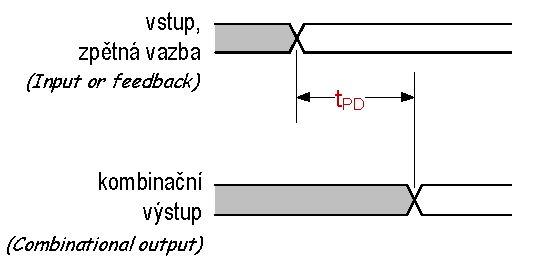
\includegraphics[width=0.9\linewidth]{PLD_timing_tpd.pdf}}                     \\
            \subfloat[Doba zpoždění po hodinovém impulzu $t_{CO}$, doba předstihu ]
              {\label{PLO:fig_PLD_timing_tsu}
              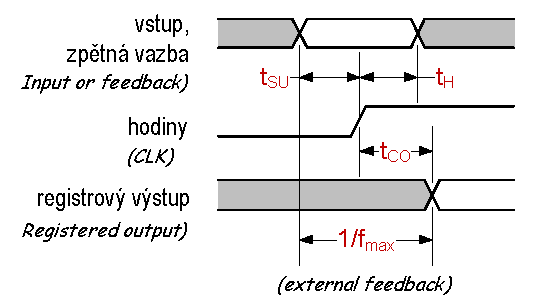
\includegraphics[width=0.9\linewidth]{PLD_timing_tsu_th_tco_fmax.pdf}}         \\
            \subfloat[ ]{\label{PLO:fig_PLD_timing_tcf}
            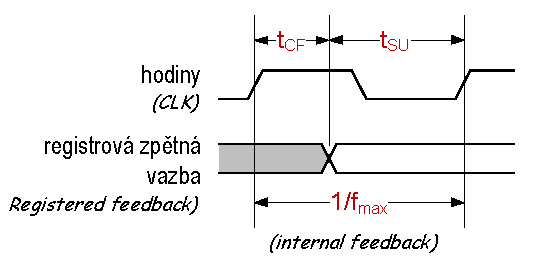
\includegraphics[width=0.9\linewidth]{PLD_timing_tsu_tcf_fmax.pdf}} 
          \end{tabular}             
          \caption{Základní dynamické parametry PLD: $t_{PD}$, $t_{CO}$, $t_{CF}$, $t_{SU}$,
                   $t_{H}$, $f_{max}$}
          \label{PLO:fig_PLD_timing}
        \end{figure}  
        
     Dynamické parametry u programovatelných logických obvodů jsou závislé na vnitř\-ních cestách 
     signálů. U obvodů \texttt{CPLD} je situace jednodušší, neboť cesty signálů jsou do jisté míry 
     pevně dány a jedná se jen o jejich výběr. Výrobci uvádějí korekční vztahy pro výše uvedené 
     doby, kterými jsou respektovány logické zátěže a způsob využití vnitřních bloků. Složitější
     situace je u obvodů \texttt{FPGA}, kde cesty signálů nejsou předem definovány a v procesu 
     návrhu budou teprve vyvtářeny. Jednotlivé doby proto musí dodatečně dopočítat návrhový systém 
     \cite[p~288]{Pinker2006}.

\printbibliography[heading=subbibliography]             
  
  %=====================================Kapitola: Úvod do tříd=========================================
  %===========================Kapitola: Jazyk VHDL==================================================
\chapter{Jazyk VHDL}
\minitoc
\newpage
  \section{Návrh číslicového obvodu}
    \subsection{Popis číslicové funkce}
      Máme-li představu o funkci a struktuře budoucího číslicového obvodu, nastupuje proces \emph{zachycení návrhu} (design
      entry, design capture), při kterém je nutné naše představy přenést do počítačem zpracovatelné formy. Tuto úlohu, lze splnit
      na růcných úrovních abstrakce \cite[s.~19]{Stastny2010}:
      \begin{itemize}
        \item \textbf{hradlové/schématické} - navrhujeme přímo kreslením schématu budoucího ovbodu. Výhodou tohoto postupu je jeho
          srozumitelnost a zachycení skuteč\-né podoby návrhu  - co máme ve schématu je to, co se realizuje. Nevýhody nicméně
          převyšují výhody. Kreslení schéma je obvykle specifické pro zvolený obvdou, protože často pužíváme struktury, které jsou
          k dispozici jen na příslušném PLD obvodu. Konverze do jiného obvou, znamená překleslení schématu. Vlastní proces
          kreslení je pomalý a únavný, protože pracujeme na nízké úrovni abstrakce - kreslíme obvod hradldo po hradle. Chceme-li
          například realizovat stavový automat, musíme nejprve zminimalizovat jeho přechodovou a výstupní funkci a pak nakreslit
          schéma. Snadno se můžeme dostat do situace, kdy je nutné kompletní překreslení. 
        \item \textbf{meziregistrových přenosů} - tzv. \texttt{RTL} (\emph{Register Transfer Level}). \texttt{RTL} popis je dnes
          standardním prostřekdem pro popis číslicové funkce. Číslicové synchronní obvody se skládají ze dvou základních typů
          logických bloků: pamě\-ťo\-vých prvků (registrů) a kombinačních funkcí. Na úrovni abstrakce, číslicový obvod popisujeme
          tak, že jednotlivé struktury popíšme pomocí těchto dvou typů logiky a doplníme informací o jejich vzájemném propojení
          (odkud, kam a přes jaké kombinančí logické funkce jsou přelévána data mezi registry). Popis obvodu je realizován v
          textové podobě pomocí zápisu ve speciálním progra\-mo\-va\-cím jazyku (\texttt{HDL} - \emph{Hardware Description
          Language}). Pro popis se používají nejčastěji jazyk \texttt{VHDL} a \texttt{Verilog}. Použití \texttt{RTL} úrovně má
          nesporné výhody: získáme technologicky nezávislý popis obvodu na relativné vysoké úrovni abstrakce, přičemž jeden řádek
          zdrojového kódu je v hardware reprezentován typicky desítkami/stovkami hradel. To zvyšuje produktivitu práce,
          zpřehledňuje vlastní návrh, zjednodušuje přenos návrhu mezi různými technologiemi a zrychluje jak vlastní návrh, tak
          pozdější opravy. Jedinou nevý\-ho\-dou je nevhodnost pro ryze asynchronní návhr, to ale není při práci s
          hrad\-lo\-vý\-mi poli omezující, neboť hradlová pole jsou určena právě pro synchronní číslicové obvody.
        \item \textbf{algoritmické} - neustále se zkracující délka návrhového cyklu spolu s rostoucí komplexitou navrhovaných
        systémů nutí návrháře používat stále vyšší úrovně abstrakce. Architektura na \texttt{RTL} úrovni je navrhována vždy s
        ohledem ke skutečnému časování obvodu a použitém paralelizmu. Systém je na této úrovni narvržen s odpovídajícím počtem
        výpočetních jednotek, řídicích bloků, sběrnic, apod. Problém nastává v okamžiku, kdy v pozdějších fázích návrhu zjistíme,
        že navržená architektura nesplňuje očekávání. Právě od\-stra\-ně\-ní informace o paralelismu a časování ze zdrojového kódu
        je přínosem \emph{algoritmické syntézy}. Funkce bloku je popsána v některém z jazyků na ''vyšší úrovni'' - např.
        \texttt{ANSI C}, \texttt{Handel-C}, \texttt{SystemC}, nebo \texttt{System Verilogu}. Příslušný syntézní nástroj pak
        dostane informaci o počtu funkčních jednotek a časování ve formě jednoduchých oemzení (například povolíme použití nejvýše
        dvou násobiček a dvou sčítaček) a na základě pžedloženého algoritmu vygeneruje \texttt{RTL} kód výsledného systému
        (datových cest i řídicích bloků). Kaž\-dá změna v architektuře je triviální - zjistíme-li, že výpočetní výkon systému je
        příliš nízký, stačí jen znovu spustit syntézní proces s jiným počtem aritmetických jednotek. Rychlost celého procesu
        umožňuje vyzkoušet celou řadu alternativ architektury a najít nejvhodnější kompromis mezi plochou a rychlostí obvodu.
        Zjednodušuje se i verifikace. Použitelnost algoritmické syntézy zatím omezuje fakt, že výsledek není tak dobrý v
        porovnání s návrhem od profesionála. 
      \end{itemize}
  \section{Úvod}
    Název VHDL představuje akronym — \texttt{VHSIC} \texttt{Hardware Description Language}. Samo označení \texttt{VHSIC} je další
    akronym představující název projektu, v rámci něhož byl jazyk VHDL zpracován, a znamená \texttt{Very High Speed Integrated
    Circuits}. I když označení \texttt{VHDL} v tomto kontextu není příliš přiléhavé, vžilo se a obecně se používá. Jazyk VHDL byl
    původně vyvinut především pro modelování a simulaci rozsáhlých systémů. Na mnoha jeho konstruktech je to znát, některé z nich
    nemají pro syntézu vůbec význam. Zde se však budeme zabývat především použitím jazyka VHDL k vytváření modelů určených pro
    syntézu číslicových systémů. České termíny budou v prvním výskytu zapsány tučně. Často tyto termíny nejsou ustálené, a proto
    budeme uvádět i jejich anglické ekvivalenty, které již většinou mají ustálenou podobu.

  \newpage
  % ----------------------------------- Základní vlastnosti jazyka VHDL ----------------------------------------------------------
  \section{Základní vlastnosti jazyka VHDL}
     \begin{itemize}
       \item Je to otevřený standard (\emph{open standard}). K jeho použití pro sestavení návrhových systémů není třeba licence
         jeho vlastníka, jako je tomu u jiných jazyků HDL (například u jazyka \texttt{ABEL}). To je jeden z důvodů, proč je tento
         jazyk v návrhových systémech často používán.
       \item Umožňuje pracovat na návrhu, aniž je předtím zvolen cílový obvod. Ten může být zvolen až v okamžiku, kdy jsou známy
         definitivní požadavky na prostředí, v němž má navrhovaný systém pracovat, a je možno cílový obvod měnit podle potřeby při
         zachování textu popisujícího systém, může být zvolen obvod \texttt{PLD} nebo \texttt{FPGA} (\emph{Device-independent
         design}).
       \item Je možno provést simulaci navrženého obvodu na základě téhož zdrojového textu, který pak bude použit pro syntézu a
         implementaci v cílovém obvodu. Zdrojový text je možno zpracovávat v různých simulátorech a v syntetizérech různých
         výrobců. Odsimulovaný text může být použit v dalších projektech s různými cílovými obvody, což je podporováno
         hierarchickou strukturou jazyka. Této vlastnosti jazyka se říká přenositelnost (\emph{portability}) kódu.
       \item V případě úspěšného zavedení výrobku na trh lze popis modelu systému v jazyku VHDL použít jako podklad pro jeho
         implementaci do obvodů \texttt{\textbf{ASIC}} vhodných pro velké série.
     \end{itemize}
     \textbf{Některé námitky proti VHDL:}
     \begin{itemize}
       \item Jazyk VHDL je dosti „upovídaný", jazykové konstrukty nejsou navrženy tak, aby zdrojový text byl stručný a při popisu
         modelu určitého systému se setkáme s opakováním bloků stejného znění. Ty je však možno snadno vytvářet využitím
         kopírování a podobných možností současných editorů.
       \item V jazyku VHDL je možno vytvořit neefektivní konstrukce, efektivnost nebo její nedostatek nemusí být na první pohled
         ze zdrojového textu patrné. To je však vlastnost i jiných jazyků vyšší úrovně a výsledná efektivnost konstrukce závisí
         nejen na kvalitě programových návrhových prostředků, ale také na zkušenosti konstruktéra (návrháře).
     \end{itemize}
  
    Základní verze jazyka VHDL byla přijata jako standard \texttt{IEEE} číslo 1076 v roce 1987. Konstrukty odpovídající tomuto
    standardu se označují jako konstrukty jazyka \texttt{VHDL-87}. Podobně jako další standardy \texttt{IEEE}, i tento standard
    se v pravidelném pětiletém intervalu aktualizuje. Upravená verze standardu byla přijata v roce 1993, odkazuje se na ni jako
    na standard \texttt{VHDL-93}.
  
    Vedle jazyka \texttt{VHDL} se setkáme také s jazykem \texttt{Verilog}, který má podobné použití. Uvádí se, že jazyk
    \texttt{VHDL} je rozšířený zejména v Evropě, zatímco \texttt{Verilog} se používá hlavně v asijských zemích. V USA se
    používají oba tyto jazyky.
    
    Vyjadřovací schopnosti jazyku VHDL jsou dány příkazy, jenž mají souběžný nebo sekvenční charakter. Některé příkazy jsou jen
    jednoho druhu, jiné mohou být obojího druhu. Toto rozlišení se týká toho, ve které části popisu se příkazy mohou používat.
    Pro stručnost budeme dále mluvit o souběžných a o sekvenčních příkazech, i když jde spíše o to, kde se tyto příkazy nacházejí
    či mohou nacházet. V následujících kapitolách jsou příkazy rozděleny do dvou velkých skupin: 
       \begin{itemize}
         \item \hyperref[Section:VHDL_soubezne_prikazy]{Souběžné příkazy} (\emph{concurrent statements}): zapisují se v
         textu jazyka mimo procesy, definice funkcí a procedur.
        \item \hyperref[Section:VHDL_sekvencni_prikazy]{Sekvenční příkazy} (\emph{sequential statements}): slouží k
         algoritmickému vyjádření popisu. Tyto příkazy mohou být zapsány jen v procesech, v definicích funkcí a procedur.
       \end{itemize}
  % ------------------------------------------------------------------------------------------------------------------------------
  \section{Logické úrovně}
   Od jazyka určeného k návrhu a modelování integrovaných obvodů očekáváme schopnost modelovat základní logické úrovně -
   \emph{log. 0} a \emph{log. 1}. Ty jsou pro jednoduché simulace postačující, ale již například pro návrh a modelování
   třístavových budičů sběrnic potřebujeme mít možnost pracovat se stavem vysoké impedance \emph{Z}. Dalším jednoduchým
   příkladem může byt modelování zkratu na sběrnici, který může vzniknout v situaci, kdy dva budiče budí jeden spoj
   opačnými logickými úrovněmi. Balíček \texttt{std\_logic\_1164} knihovny \texttt{IEEE} pro tyto účely zavádí
   \emph{devítistavovou logiku}. 
   
   \begin{itemize}
     \item 'U': uninitialized. This signal hasn't been set yet.
     \item 'X': unknown. Impossible to determine this value/result.
     \item '0': logic 0
     \item '1': logic 1
     \item 'Z': High Impedance
     \item 'W': Weak signal, can't tell if it should be 0 or 1.
     \item 'L': Weak signal that should probably go to 0
     \item 'H': Weak signal that should probably go to 1
     \item '-': Don't care.
   \end{itemize}
   
   Všimněme si, že tato knihovna je připojena všemi ukázkovými kódy. Logický signál, který má popsaných hodnot nabývat, je pak
   definován jako signál typu \texttt{std\_logic}, nebo \texttt{std\_logic\_vector} pokud se jedná o sběrnici. Pomocí nich
   modelujeme standardní propojení logických prvků, tj. ''obyčený kus drátu''.
   \cite[s.~51]{Stastny2010}
  \section{Souběžné příkazy} \label{Section:VHDL_soubezne_prikazy}
  \newpage
  \section{Sekvenční příkazy}\label{Section:VHDL_sekvencni_prikazy} 
  \section{Technologicky nezávislá část návrhu}
    V následujícím textu jsou uvedeny základní způsoby popisu chování sekvenčních (např. klopné obvody) a kombinačních obvodů.
    Klopné obvody jsou rozdělovány na \textbf{hranově citlivé} a \textbf{úrovňově citlivé}. Je možné je popsat jako
    \emph{jednobitové paměti}. Hranově citlivý klopný obvod je obvod řízený změnou na vstupu synchronizace (\emph{clock input}).
    Bývá označován "\emph{flip-flop}".  Úrovňově citlivý klopný obvod je nazýván v české terminologii \emph{zdrž}. Obvykle je však
    srozumitelný anglický název "\emph{latch}".
  
    \subsection{Dynamicky řízené sekvenční obvody}
      Obvody řízené změnou signálu na vstupu synchronizace jsou ve VHDL popisovány použitím příkazu process a podmíněného příkazu
      \lstinline[basicstyle=\ttfamily]!if!. V podmíně\-ném příkazu jsou rozlišovány události
      (\lstinline[basicstyle=\ttfamily]!events!), které znamenají vzestupnou hranu nebo sestupnou hranu signálu na vstupu
      synchronizace. Při popisu je možné použít dvou různých zápisů, ve kterých se objevuje atribut události synchronizačního
      signálu \lstinline[basicstyle=\ttfamily]!clk clk'event! nebo volání funkce.
      \begin{itemize}
        \item \lstinline[basicstyle=\ttfamily]!(clk'event and clk='1')!  	 vzestupná hrana signálu
        \item \lstinline[basicstyle=\ttfamily]!(clk'event and clk='0')!    sestupná hrana signálu
        \item \lstinline[basicstyle=\ttfamily]!rising_edge(clk)!		     voláni funkce vzestupné hrany
        \item \lstinline[basicstyle=\ttfamily]!falling_edge(clk)!		     voláni funkce sestupné hrany
      \end{itemize}
      Uvedené příklady ukazují možnosti vyjádření vzestupné a sestupné hrany ve VHDL. Vyjádření pomocí atributu je častěji
      používané, protože tento konstrukt je rozeznatelný při syntéze obvodového řešení. Nicméně použití volání funkce je
      výhodnější při simulaci, protože nastává pouze při změně signálu \lstinline[basicstyle=\ttfamily]!clk! z $0\rightarrow1$ a
      z $1\rightarrow0$, ale ne z $X\rightarrow1$ nebo z $0\rightarrow X$, které nepředstavují platný přechod z jednoho stavu do
      druhého. Devět hodnot signálu, které jsou označované jako \lstinline[basicstyle=\ttfamily]!std_logic! jsou určeny k
      modelování poruchových stavů logické sítě. Jsou to hodnoty \emph{'U','X','0','1'¸'Z','W','L','H','-'}.
 
        \subsection{Staticky řízené sekvenční obvody}
          V následujících odstavcích jsou popisovány klopné obvody řízené úrovní synchronizačního signálu, které jsou známé pod
          názvem \textbf{zdrž} (\emph{latch}).
    
    \subsection{Kombinační obvody} 

  \section{Knihovna LPM}
    Knihovna \textbf{LPM} (angl. \emph{Library of Parametrized module}) obsahuje parametrizovatelné moduly jako jsou hrada,
    čítače, multiplexory, klopné obvody, aritmetické a paměťové funkce. 
  
    Standard \texttt{LPM} byl navržen v roce 1990 jako jedna z monžností pro efektivní návrh číslicových systémů do odlišných
    technologií, jako jsou např. obvody PLD, hradlová pole a standardní buňky. Předběžná verze standardu vyšla v roce 1991, další
    úprava předběžné verze pak v roce 1992.
    Standard byl přijat organizací \texttt{EIA} (angl. \emph{Electronic Industires Alliance}) v dubnu roku 1993 jako doplněk do
    standardu \texttt{EDIF}.
  
    \texttt{EDIF} je formát pro přenos návrhu mezi návrhovými nástroji různých výrobců. Formát \texttt{EDIF} popisuje syntaxi,
    která reprezentuje logický netlist. \texttt{LPM} do něj pak přidává množinu funkcí, která popisuje logické operace netlistu.
    Před rozšířením o \texttt{LPM} musel každý \texttt{EDIF} netlit typicky obsahovat technologicky specifické logické funkce,
    které zabraňovaly tomu, aby byl návrh ve větší míře nezávislý na cílové technologii \cite[s.~72]{Pinker2006}. 
  
    \subsection{Posuvný registr - lpm shiftreg}
  
    \begin{table} 
      \begin{tabular}{|c|p{3.5cm}|p{8cm}|}
        \hline
           \rowcolor{CornflowerBlue} {\textbf{Jméno}}              & {\textbf{Popis}}          & {\textbf{komentář}} \\
        \hline\hline       
           \texttt{data[]}   & Data input to the shift register    & Šířku registru určuje parametr \texttt{LPM\_WIDTH}. \\
        \hline   
           \texttt{clock}    & Positive-edge-triggered clok        & Vstup hodinového signálu. \\
        \hline     
           \texttt{enable}   & Clock enable input                  & Blokuje hodinový signál. \\
        \hline      
           \texttt{shiftin}  & Serial shift data input             & Pro funkci je nutné použit alespoň jeden ze signálů
           \texttt{data[]}, \texttt{aset}, \texttt{aclr}, \texttt{sset}, \texttt{sclr}, a/nebo
                                                                  \texttt{shiftin}.  \\
        \hline    
           \texttt{load}     & Synchronous parallel load           & (1) load operation (podmínka: \texttt{enable} = 1); (0) shift
           operation (výchozí). \\
        \hline    
           \texttt{aclr}     & Asynchronnous clear input           & Signál \texttt{aclr} má vyšší prioritu než signál
           \texttt{aset}.  \\
        \hline    
           \texttt{aset}     & Asynchronnous set input             & Naplní registr \texttt{g[]} hodnotou \texttt{LPM\_AVALUE} \\
        \hline 
           \texttt{sclr}     & Synchronous clear input             & Signál \texttt{sclr} má vyšší prioritu než signál
           \texttt{sset}.  \\
        \hline  
           \texttt{sset}     & Syncrhonous set input               & Naplní registr \texttt{g[]} hodnotou \texttt{LPM\_SVALUE} \\
        \hline  
           \texttt{q[]}      & Data output from the shift register & Šířku registru určuje parametr \texttt{LPM\_WIDTH}. Vyžaduje
           \texttt{shiftout}.  \\
        \hline 
           \texttt{shiftout} & Serial shift data output            & Vyžaduje registr \texttt{q[]}. \\
        \hline                                                           
      \end{tabular}
      \caption{Popis portů komponenty \texttt{lpm\_shiftreg}.}
      \label{VHDL:tab_lpm_shiftreg}       
    \end{table}
    
    %---------------------------------------------------------------
    \lstinputlisting{../src/PLO/LPM/lpm_shiftreg.vhd}
    %---------------------------------------------------------------  